\chapter{Surface Fluxes}



%%%%%%%%%%%%%%%%%%%%%%%%%%%%%%%%%%%%%%%%%%%%%%%%%%%%%%%%%%%%%%%
\section{Input}
%%%%%%%%%%%%%%%%%%%%%%%%%%%%%%%%%%%%%%%%%%%%%%%%%%%%%%%%%%%%%%%

\subsection{Parameters}


\begin{center}
\begin{longtable}{|p {3.4 cm}|p {4.7 cm}|p {1. cm}|p{0.8 cm}|p{1.4 cm}|p{0.8 cm}|p{1.3 cm}|}
\hline
\textbf{Keyword} & \textbf{Description} & \textbf{M. U.} & \textbf{range} & \textbf{Default Value} & \textbf{Sca / Vec} & \textbf{Logical / Numeric} \\ \hline
\endfirsthead
\hline
\multicolumn{7}{| c |}{continued from previous page} \\
\hline
\textbf{Keyword} & \textbf{Description} & \textbf{M. U.} & \textbf{range} & \textbf{Default Value} & \textbf{Sca / Vec} & \textbf{Log / Num} \\ \hline
\endhead
\hline
\multicolumn{7}{| c |}{{continued on next page}}\\ 
\hline
\endfoot
\endlastfoot
\hline
LWinParameterization \index{LWinParameterization} & Which formula for incoming longwave radiation:  1 (Brutsaert, 1975), 2 (Satterlund, 1979), 3 (Idso, 1981), 4(Idso+Hodges),  5 (Koenig-Langlo \& Augstein, 1994), 6 (Andreas \& Ackley, 1982), 7 (Konzelmann, 1994), 8 (Prata, 1996), 9 (Dilley 1998) &  & 1, 2, .., 9 & 9 & sca & opt \\ \hline
MoninObukhov \index{MoninObukhov} & Atmospherical stability parameter: 1 stability and instability considered, 2 stability not considered, 3 instability not considered, 4 always neutrality &  &  & 1 & sca & num \\ \hline
Surroundings & Yes(1), No(0) & - &  & 0 & sca & opt \\ \hline
{\bf NumLandCoverTypes} \index{NumLandCoverTypes} & Number of Classes of land cover. Each land cover type corresponds to a particular land-cover state, described by a specific set of values of the parameters listed 
below. Each set of land cover parameters will be distributively assigned according to the land cover map, which relates each pixel with a land cover type number. This number corresponds to the number of component in the numerical vector that is assigned to any land cover parameters listed below. & - & 1, inf & 1 & sca & num \\ \hline
\caption{Keywords of parameters regarding the surface energy fluxes calculation}
\label{surfaceenergyfluxes1d_numeric}
\end{longtable}
\end{center}


\begin{center}
\begin{longtable}{|p {3.4 cm}|p {4.7 cm}|p {1. cm}|p{0.8 cm}|p{1.4 cm}|p{0.8 cm}|p{1.3 cm}|}
\hline
\textbf{Keyword} & \textbf{Description} & \textbf{M. U.} & \textbf{range} & \textbf{Default Value} & \textbf{Sca / Vec} & \textbf{Str / Num / Opt} \\ \hline
\endfirsthead
\hline
\multicolumn{7}{| c |}{continued from previous page} \\
\hline
\textbf{Keyword} & \textbf{Description} & \textbf{M. U.} & \textbf{range} & \textbf{Default Value} & \textbf{Sca / Vec} & \textbf{Str / Num / Opt} \\ \hline
\endhead
\hline
\multicolumn{7}{| c |}{{continued on next page}}\\ 
\hline
\endfoot
\endlastfoot
\hline
SoilRoughness \index{SoilRoughness} & Roughness length of soil surface & mm & 0, 1000 & 10 & vec & num \\ \hline
SoilAlbVisDry \index{SoilAlbVisDry} & Ground surface albedo without snow in the visible - dry & - & 0, 1 & 0.2 & vec & num \\ \hline
SoilAlbNIRDry \index{SoilAlbNIRDry} & Ground surface albedo without snow in the near infrared - dry & - & 0, 1 & 0.2 & vec & num \\ \hline
SoilAlbVisWet \index{SoilAlbVisWet} & Ground surface albedo without snow in the visible - saturated & - & 0, 1 & 0.2 & vec & num \\ \hline
SoilAlbNIRWet \index{SoilAlbNIRWet} & Ground surface albedo without snow in the near infrared - saturated & - & 0, 1 & 0.2 & vec & num \\ \hline
SoilEmissiv \index{SoilEmissiv} & Ground surface emissivity & - & 0, 1 & 0.96 & vec & num \\ \hline
\caption{Keywords of land cover characteristics affecting surface energy fluxes that may be set in geotop.inpts. Each parameter may be given in input as a vector, each component representing the value corresponding to the LandCoverMapFile value identified by the vector index}
\label{surfluxes_landcover}
\end{longtable}
\end{center}

\section{Numerics}
\begin{center}
\begin{longtable}{|p {3.5 cm}|p {5 cm}|p {1 cm}|p{1 cm}|p{1.1 cm}|p{1.cm}|p{1 cm}|}
\hline
\textbf{Keyword} & \textbf{Description} & \textbf{M. U.} & \textbf{range} & \textbf{Default Value} & \textbf{Scalar / Vector} & \textbf{Logical / Numeric} \\ \hline
\endfirsthead
\hline
\multicolumn{7}{| c |}{continued from previous page} \\
\hline
\textbf{Keyword} & \textbf{Description} & \textbf{M. U.} & \textbf{range} & \textbf{Default Value} & \textbf{Sca / Vec} & \textbf{Log / Num} \\ \hline
\endhead
\hline
\multicolumn{7}{| c |}{{continued on next page}}\\ 
\hline
\endfoot
\endlastfoot
\hline
BusingerMaxIter \index{BusingerMaxIter} & Max number of iterations for Monin-Obulhov stability algorithm -Businger parameterization (surface energy balance equation) & - &  & 5 & sca & num \\ \hline
\caption{Keywords of input numeric parameters for the energy equation regarding vegetation routines settable in geotop.inpts}
\label{numeric1d_num_sur}
\end{longtable}
\end{center}


%%%%%%%%%%%%%%%%%%%%%%%%%%%%%%%%%%%%%%%%%%%%%%%%%%%%%%%%%%%%%%%
\section{Output}
%%%%%%%%%%%%%%%%%%%%%%%%%%%%%%%%%%%%%%%%%%%%%%%%%%%%%%%%%%%%%%%

\subsection{Point}

\subsubsection{Files}

\begin{center}
\begin{longtable}{|p {3.3 cm}|p {9 cm}|}
\hline
\textbf{Keyword} & \textbf{Description}  \\ \hline
\endfirsthead
\hline
\multicolumn{2}{| c |}{continued from previous page} \\
\hline
\textbf{Keyword} & \textbf{Description}   \\ \hline
\endhead
\hline
\multicolumn{2}{| c |}{{continued on next page}}\\ 
\hline
\endfoot
\endlastfoot
\hline
PointOutputFile \index{PointOutputFile} & name of the file providing the properties for the simulation point \\ \hline
PointOutputFileWriteEnd \index{PointOutputFileWriteEnd} & name of the output file providing the Point values written just once at the end \\ \hline
\caption{Keywords of file related to point output variables}
\label{veget_file}
\end{longtable}
\end{center}

\subsubsection{Headers}

\begin{center}
\begin{longtable}{|p {3.5 cm}|p {7 cm}|p {2 cm}|p {2 cm}|}
\hline
\textbf{Keyword} & \textbf{Description} & \textbf{Associated file}  \\ \hline
\endfirsthead
\hline
\multicolumn{4}{| c |}{continued from previous page} \\
\hline
\textbf{Keyword} & \textbf{Description} & \textbf{Associated file}  \\ \hline
\endhead
\hline
\multicolumn{4}{| c |}{{continued on next page}}\\ 
\hline
\endfoot
\endlastfoot
\hline
HeaderSurfaceEBPoint \index{HeaderSurfaceEBPoint} & column name in the file PointOutputFile for the variable SurfaceEBPoint & PointOutputFile  \\ \hline
HeaderSoilHeatFluxPoint \index{HeaderSoilHeatFluxPoint} & column name in the file PointOutputFile for the variable SoilHeatFluxPoint & PointOutputFile  \\ \hline
HeaderSWinPoint \index{HeaderSWinPoint} & column name in the file PointOutputFile for the variable SWinPoint & PointOutputFile  \\ \hline
HeaderSWbeamPoint \index{HeaderSWbeamPoint} & column name in the file PointOutputFile for the variable SWbeamPoint & PointOutputFile  \\ \hline
HeaderSWdiffPoint \index{HeaderSWdiffPoint} & column name in the file PointOutputFile for the variable SWdiffPoint & PointOutputFile  \\ \hline
HeaderLWinPoint \index{HeaderLWinPoint} & column name in the file PointOutputFile for the variable LWinPoint & PointOutputFile  \\ \hline
HeaderLWinMinPoint \index{HeaderLWinMinPoint} & column name in the file PointOutputFile for the variable LWinMinPoint & PointOutputFile  \\ \hline
HeaderLWinMaxPoint \index{HeaderLWinMaxPoint} & column name in the file PointOutputFile for the variable LWinMaxPoint & PointOutputFile  \\ \hline
HeaderSWNetPoint \index{HeaderSWNetPoint} & column name in the file PointOutputFile for the variable SWNetPoint & PointOutputFile  \\ \hline
HeaderLWNetPoint \index{HeaderLWNetPoint} & column name in the file PointOutputFile for the variable LWNetPoint & PointOutputFile  \\ \hline
HeaderHPoint \index{HeaderHPoint} & column name in the file PointOutputFile for the variable HPoint & PointOutputFile  \\ \hline
HeaderLEPoint \index{HeaderLEPoint} & column name in the file PointOutputFile for the variable LEPoint & PointOutputFile  \\ \hline
HeaderQSurfPoint \index{HeaderQSurfPoint} & column name in the file PointOutputFile for the variable specific humidity near the soil surface & PointOutputFile  \\ \hline
HeaderQAirPoint \index{HeaderQAirPoint} & column name in the file PointOutputFile for the variable specific humidity of the air & PointOutputFile  \\ \hline
HeaderLObukhovPoint \index{HeaderLObukhovPoint} & column name in the file PointOutputFile for the variable LObukhovPoint & PointOutputFile  \\ \hline
HeaderSWupPoint \index{HeaderSWupPoint} & column name in the file PointOutputFile for the variable SWupPoint & PointOutputFile  \\ \hline
HeaderLWupPoint \index{HeaderLWupPoint} & column name in the file PointOutputFile for the variable LWupPoint & PointOutputFile  \\ \hline
HeaderHupPoint \index{HeaderHupPoint} & column name in the file PointOutputFile for the variable HupPoint & PointOutputFile  \\ \hline
HeaderLEupPoint \index{HeaderLEupPoint} & column name in the file PointOutputFile for the variable LEupPoint & PointOutputFile  \\ \hline
\caption{Keywords defining the headers to personalize for the output related to surface flux in the PointOutputFile}
\label{surenfluxheader_data}
\end{longtable}
\end{center}



\subsubsection{Parameters}

\begin{center}
\begin{longtable}{|p {3.2 cm}|p {4.8 cm}|p {1 cm}|p{1.4 cm}|p{1.5 cm}|p{1. cm}|p{1 cm}|}
\hline
\textbf{Keyword} & \textbf{Description} & \textbf{M. U.} & \textbf{range} & \textbf{Default Value} & \textbf{Sca / Vec} & \textbf{Log / Num} \\ \hline
\endfirsthead
\hline
\multicolumn{7}{| c |}{continued from previous page} \\
\hline
\textbf{Keyword} & \textbf{Description} & \textbf{M. U.} & \textbf{range} & \textbf{Default Value} & \textbf{Sca / Vec} & \textbf{Log / Num} \\ \hline
\endhead
\hline
\multicolumn{7}{| c |}{{continued on next page}}\\ 
\hline
\endfoot
\endlastfoot
\hline
DefaultPoint \index{DefaultPoint} & 0: use personal setting, 1:use default & - & 0, 1 & 1 & sca & opt \\ \hline
DtPlotPoint \index{DtPlotPoint} & Plotting Time step (in hour) of THE OUTPUT FOR SPECIFIED PIXELS (0 means the it is not plotted) & h & 0, inf & 0 & vec & num \\ \hline
DatePoint \index{DatePoint} & column number in which one would like to visualize the Date12[DDMMYYYY hhmm]    	 & - & 1, 76 & -1 & sca & num \\ \hline
JulianDayFromYear0Point \index{JulianDayFromYear0Point} & column number in which one would like to visualize the JulianDayFromYear0[days]   	 & - & 1, 76 & -1 & sca & num \\ \hline
TimeFromStartPoint \index{TimeFromStartPoint} & column number in which one would like to visualize the TimeFromStart[days]  & - & 1, 76 & -1 & sca & num \\ \hline
PeriodPoint \index{PeriodPoint} & column number in which one would like to visualize the Simulation\_Period & - & 1, 76 & -1 & sca & num \\ \hline
RunPoint \index{RunPoint} & column number in which one would like to visualize the Run	 & - & 1, 76 & -1 & sca & num \\ \hline
IDPointPoint \index{IDPointPoint} & column number in which one would like to visualize the IDpoint  & - & 1, 76 & -1 & sca & num \\ \hline
TsurfPoint \index{TsurfPoint} & column number in which one would like to visualize the Tsurface[\textcelsius]     & - & 1, 76 & -1 & sca & num \\ \hline
SurfaceEBPoint \index{SurfaceEBPoint} & column number in which one would like to visualize the Surface\_Energy\_balance [W/m$^{2}$]     & - & 1, 76 & -1 & sca & num \\ \hline
SoilHeatFluxPoint \index{SoilHeatFluxPoint} & column number in which one would like to visualize the Soil\_heat\_flux[W/m$^{2}$]      & - & 1, 76 & -1 & sca & num \\ \hline
SWinPoint \index{SWinPoint} & column number in which one would like to visualize the SWin[W/m$^{2}$]   & - & 1, 76 & -1 & sca & num \\ \hline
SWbeamPoint \index{SWbeamPoint} & column number in which one would like to visualize the SWbeam[W/m$^{2}$]    & - & 1, 76 & -1 & sca & num \\ \hline
SWdiffPoint \index{SWdiffPoint} & column number in which one would like to visualize the SWdiff[W/m$^{2}$]   & - & 1, 76 & -1 & sca & num \\ \hline
LWinPoint \index{LWinPoint} & column number in which one would like to visualize the LWin[W/m$^{2}$]  & - & 1, 76 & -1 & sca & num \\ \hline
LWinMinPoint \index{LWinMinPoint} & column number in which one would like to visualize the LWin\_min[W/m$^{2}$]  & - & 1, 76 & -1 & sca & num \\ \hline
LWinMaxPoint \index{LWinMaxPoint} & column number in which one would like to visualize the LWin\_max[W/m$^{2}$] & - & 1, 76 & -1 & sca & num \\ \hline
SWNetPoint \index{SWNetPoint} & column number in which one would like to visualize the SWnet[W/m$^{2}$]      & - & 1, 76 & -1 & sca & num \\ \hline
LWNetPoint \index{LWNetPoint} & column number in which one would like to visualize the LWnet[W/m$^{2}$]      & - & 1, 76 & -1 & sca & num \\ \hline
HPoint \index{HPoint} & column number in which one would like to visualize the H[W/m$^{2}$]       & - & 1, 76 & -1 & sca & num \\ \hline
EvapSurfacePoint \index{EvapSurfacePoint} & column number in which one would like to visualize the Evap\_surface[mm]   & - & 1, 76 & -1 & sca & num \\ \hline
LEPoint \index{LEPoint} & column number in which one would like to visualize the LE[W/m$^{2}$]      & - & 1, 76 & -1 & sca & num \\ \hline
QSurfPoint \index{QSurfPoint} & column number in which one would like to visualize the specific humidity at the surface (grams vapour/grams air)  & - & 1, 76 & -1 & sca & num \\ \hline
QAirPoint \index{QAirPoint} & column number in which one would like to visualize the specific humidity at air (grams vapour/grams air)  & - & 1, 76 & -1 & sca & num \\ \hline
LObukhovPoint \index{LObukhovPoint} & column number in which one would like to visualize the LObukhov[m] & - & 1, 76 & -1 & sca & num \\ \hline
SWupPoint \index{SWupPoint} & column number in which one would like to visualize the SWup[W/m$^{2}$]    & - & 1, 76 & -1 & sca & num \\ \hline
LWupPoint \index{LWupPoint} & column number in which one would like to visualize the LWup[W/m$^{2}$]    & - & 1, 76 & -1 & sca & num \\ \hline
HupPoint \index{HupPoint} & column number in which one would like to visualize the Hup[W/m$^{2}$]     & - & 1, 76 & -1 & sca & num \\ \hline
LEupPoint \index{LEupPoint} & column number in which one would like to visualize the LEup[W/m$^{2}$]    & - & 1, 76 & -1 & sca & num \\ \hline
\caption{Keywords defining which parameter to print on the PointOutputFile}
\label{surfluxpoint_numeric}
\end{longtable}
\end{center}




\subsection{Maps}
\subsubsection{Parameters}

\begin{center}
\begin{longtable}{|p {3. cm}|p {3.5 cm}|p {2.5 cm}|p{1.7 cm}|p{1. cm}|p{1. cm}|p{1. cm}|}
\hline
\textbf{Keyword} & \textbf{Description} & \textbf{M. U.} & \textbf{range} & \textbf{Default Value} & \textbf{Sca / Vec}  \\ \hline
\endfirsthead
\hline
\multicolumn{7}{| c |}{continued from previous page} \\
\hline
\textbf{Keyword} & \textbf{Description} & \textbf{M. U.} & \textbf{range} & \textbf{Default Value} & \textbf{Sca / Vec}  \\ \hline
\endhead
\hline
\multicolumn{7}{| c |}{{continued on next page}}\\ 
\hline
\endfoot
\endlastfoot
\hline
OutputSurfEBALMaps \index{OutputSurfEBALMaps} & frequency (h) of printing of the results of the Surface energy balance maps & h &  & 0 & sca \\ \hline
\caption{Keywords for parameters of printing details for surface energy balance maps}
\label{out_map_surfeb}
\end{longtable}
\end{center}

\subsubsection{File}

\begin{center}
\begin{longtable}{|p {6. cm}|p {7 cm}|p {2 cm}|p {2 cm}|}
\hline
\textbf{Keyword} & \textbf{Description}   \\ \hline
\endfirsthead
\hline
\multicolumn{4}{| c |}{continued from previous page} \\
\hline
\textbf{Keyword} & \textbf{Description}   \\ \hline
\endhead
\hline
\multicolumn{4}{| c |}{{continued on next page}}\\ 
\hline
\endfoot
\endlastfoot
\hline
RadiationMapFile \index{RadiationMapFile} & name of the output file providing the Radiation map (all the type of radiations)   \\ \hline
NetRadiationMapFile \index{NetRadiationMapFile} & name of the output file providing the Net Radiation map   \\ \hline
InLongwaveRadiationMapFile \index{InLongwaveRadiationMapFile} & name of the output file providing the LW Radiation map   \\ \hline
NetLongwaveRadiationMapFile \index{NetLongwaveRadiationMapFile} & name of the output file providing the Net LW  Radiation map   \\ \hline
NetShortwaveRadiationMapFile \index{NetShortwaveRadiationMapFile} & name of the output file providing the Net SW  Radiation map   \\ \hline
InShortwaveRadiationMapFile \index{InShortwaveRadiationMapFile} & name of the output file providing the Swin  Radiation map   \\ \hline
DirectInShortwaveRadiationMapFile \index{DirectInShortwaveRadiationMapFile} & name of the output file providing the Swdir  Radiation map   \\ \hline
ShadowFractionTimeMapFile \index{ShadowFractionTimeMapFile} & name of the output file providing the map of the  fraction of Shadow in the time   \\ \hline
SurfaceHeatFluxMapFile \index{SurfaceHeatFluxMapFile} & name of the output file providing the Surface heat flux  map   \\ \hline
SurfaceSensibleHeatFluxMapFile \index{SurfaceSensibleHeatFluxMapFile} & name of the output file providing the Surface sensible heat flux  map   \\ \hline
SurfaceLatentHeatFluxMapFile \index{SurfaceLatentHeatFluxMapFile} & name of the output file providing the Surface latent  heat flux  map   \\ \hline
SpecificPlotSurfaceHeatFluxMapFile \index{SpecificPlotSurfaceHeatFluxMapFile} & name of the output file providing the surface heat flux map at high temporal resolution during specific days   \\ \hline
SpecificPlotTotalSensibleHeatFluxMapFile \index{SpecificPlotTotalSensibleHeatFluxMapFile} & name of the output file providing the total sensible heat flux map at high temporal resolution during specific days   \\ \hline
SpecificPlotTotalLatentHeatFluxMapFile \index{SpecificPlotTotalLatentHeatFluxMapFile} & name of the output file providing the total latent heat flux map at high temporal resolution during specific days   \\ \hline
SpecificPlotSurfaceSensibleHeatFluxMapFile \index{SpecificPlotSurfaceSensibleHeatFluxMapFile} & name of the output file providing the surface sensible heat flux map at high temporal resolution during specific days   \\ \hline
SpecificPlotSurfaceLatentHeatFluxMapFile \index{SpecificPlotSurfaceLatentHeatFluxMapFile} & name of the output file providing the surface latent heat flux map at high temporal resolution during specific days   \\ \hline
SpecificPlotIncomingShortwaveRadMapFile \index{SpecificPlotIncomingShortwaveRadMapFile} & name of the output file providing the Swin flux map at high temporal resolution during specific days   \\ \hline
SpecificPlotNetSurfaceShortwaveRadMapFile \index{SpecificPlotNetSurfaceShortwaveRadMapFile} & name of the output file providing the surface Swnet flux map at high temporal resolution during specific days   \\ \hline
SpecificPlotIncomingLongwaveRadMapFile \index{SpecificPlotIncomingLongwaveRadMapFile} & name of the output file providing the Lwin flux map at high temporal resolution during specific days   \\ \hline
SpecificPlotNetSurfaceLongwaveRadMapFile \index{SpecificPlotNetSurfaceLongwaveRadMapFile} & name of the output file providing the surface Lwnet map at high temporal resolution during specific days   \\ \hline
% &\\
%\hline
\caption{Keywords of output map files related to surface fluxes settable in geotop.inpts }
\label{surenfluxmap}
\end{longtable}
\end{center}


%%%%%%%%%%%%%%%%%%%%%%%%%%%%%%%%%%%%%%%%%%%%%%%%%%%%%%%%%%%%%%%
\section{Values of reference}
%%%%%%%%%%%%%%%%%%%%%%%%%%%%%%%%%%%%%%%%%%%%%%%%%%%%%%%%%%%%%%%


\begin{table}[!h]
\begin{footnotesize}
\begin{center}
\begin{tabular}{lll}
  \hline
  \hline
  \textsl{Surface description}	 	& \textsl{roughness $z_0$ [mm]}	  	& \textsl{Reference} \\
  \hline
    Mud flats, ice			&   0.01 			& \citet{sutton1953micrometeorology} \\ 
    Smooth tarmac			&   0.02 			& \citet{bradley1968micrometeorological}) \\
    Large water surfaces		&   0.1 - 0.6			& Numerous references \\
    Grass (lawn up to 1 cm)		&   1 				& \citet{sutton1953micrometeorology} \\
    Grass (artificial, 7.5 cm high)	&   10 				& \citet{chamberlain1966transport}) \\
    Grass (thick up to 10 cm high)	&   23 				& \citet{sutton1953micrometeorology} \\
    Grass (thin up to 50 cm)		&   50 				& \citet{sutton1953micrometeorology} \\
    Trees (10-15 m high)		&   400-700 			& \citet{fichtl1970longitudinal} \\
    Large city				&   1650 			& \citet{yamamoto1964profiles}\\
\hline
\hline
\end{tabular}
\textsl{\caption{Example of roughness parameters for various surfaces \cite{brutsaert1982evaporation}}}\label{tu}
 \end{center}
\end{footnotesize}
\end{table}


Radiative proprieties of natural materials p.13 Boundary Layer Climates - T.R.Oke
\begin{table}[!h]
\begin{footnotesize}
\begin{center}
\begin{tabular}{l|lll}
  \hline
  \hline
  \textsl{Surface}         	& \textsl{Remarks}  	& \textsl{Albedo} 	 & \textsl{Emissivity}  \\
 \textsl{}   			& \textsl{}   		& \textsl{$\alpha$}      & \textsl{$ \varepsilon$}    \\
  \hline
   Soil	 		   	& Dark, wet 		&  0.05 - 		& 0.98 - \\
   	 		   	& Light, dry	 	&  0.40 		& 0.90 \\
   Desert 	 	   	&  			&  0.20 - 0.45 		& 0.84 - 0.91 \\    
   Grass	 	   	& Long (1.0 m)		&  0.16 - 		& 0.90 - \\             
				& Short (0.02 m		&  0.26 		& 0.95\\
   Agrigultural crops,  	&  			&  0.18 - 		& 0.90 - \\    
   tundra		  	&  			&  0.25 		& 0.99\\    
   Orchards	 		&  			&  0.15 - 0.20 		& \\        
   Forest			&  			&  			& \\              
   \hspace{0.5cm} Deciduos	&  Bare 		&  0.15 - 		& 0.97 - \\  
				&  Leaved		&  0.20 		& 0.98 \\               
   \hspace{0.5cm} Coniferous	&  			&  0.05 - 0.15 		& 0.97 - 0.99 \\         
   Water	 		&  Small zenith angle 	&  0.03 - 0.10 		& 0.92 - 0.97 \\  
				&  Large zenith angle 	&  0.10 - 1.00 		& 0.92 - 0.97 \\             
   Snow	 			&  Old			&  0.40 - 		& 0.82 - \\            
   	 			&  Fresh		&  0.95 		& 0.99 \\ 
  Ice	 			&  Sea 			&  0.30 - 0.45 		& 0.92 - 0.97 \\           
  	 			&  Glacier 		&  0.20 - 0.40 		& \\           
  \hline
  \hline
\end{tabular}
\textsl{\caption{Radiative proprieties of natural materials}}\label{ddd}
 \end{center}
\end{footnotesize}
\end{table}




Example of roughness parameters for various surfaces - Evaporation into the Atmosphere, Wilfried Brutsaert, 1984
\begin{table}[!h]
\begin{footnotesize}
\begin{center}
\begin{tabular}{lll}
  \hline
  \hline
  \textsl{Surface description}	 	& \textsl{z\_{0}(cm)}	  	& \textsl{Reference} \\
  \hline
    Mud flats, ice			&   0.001 			& Sutton (1953) \\ 
    Smooth tarmac			&   0.002 			& Bradley (1968) \\
    Large water surfaces		&   0.01 - 0.06			& Numerous references \\
    Grass (lawn up to 1 cm)		&   0.1 			& Sutton (1953) \\
    Grass (artificial, 7.5 cm high)	&   1.0 			& Chamberlain (1966) \\
    Grass (thick up to 10 cm high)	&   2.3 			& Sutton (1953) \\
    Grass (thin up to 50 cm)		&   5 				& Sutton (1953) \\
    Trees (10-15 m high)		&   40-70 			& Fichtl and McVehil (1970) \\
    Large city				&   165 			& Yamamoto and Shimanuki (1964)\\
\hline
\hline
\end{tabular}
\textsl{\caption{Example of roughness parameters for various surfaces (Evaporation into the Atmosphere, Wilfried Brutsaert, 1984)}}\label{}
 \end{center}
\end{footnotesize}
\end{table}



%\begin{figure}[!h]
%\begin{center}
%  \begin{minipage}[c]{.60\textwidth}
%    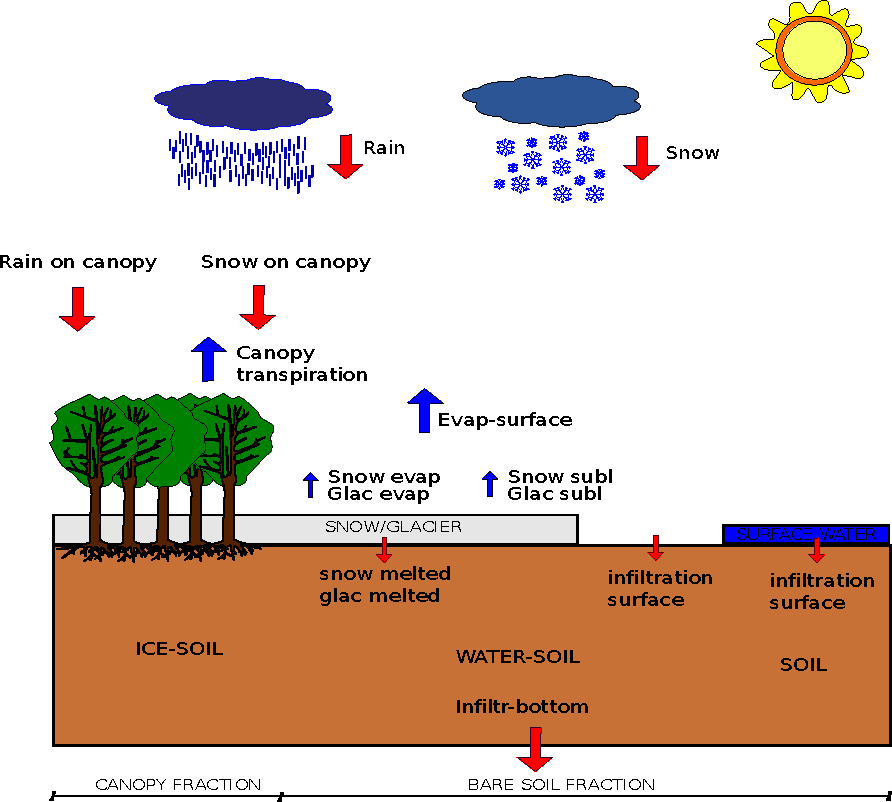
\includegraphics[width=1\textwidth]{./images/pic_surFlux/water_fluxes.pdf}
%    \textsl{\caption{Water fluxes} \label{}}
%  \end{minipage}
%\end{center}
%\end{figure}

%
%\begin{figure}[!h]
%\begin{center}
%  \begin{minipage}[c]{.60\textwidth}
%    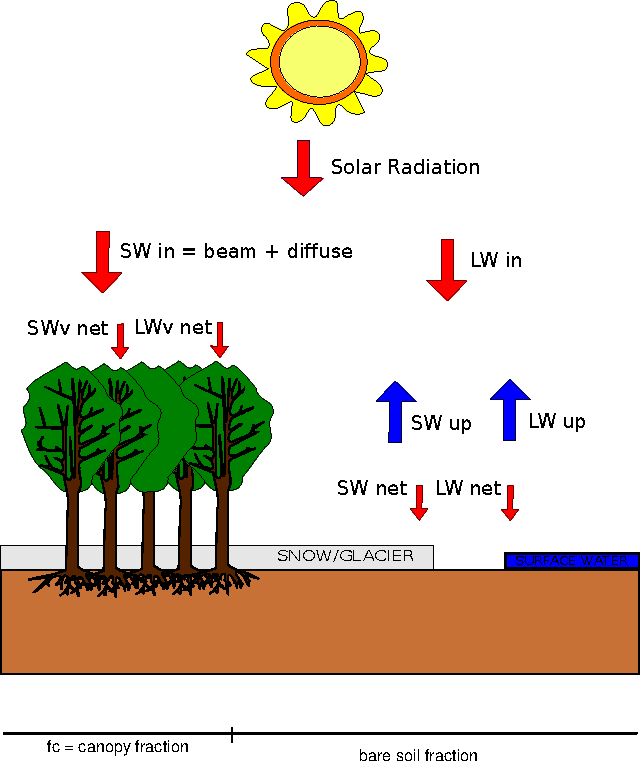
\includegraphics[width=1\textwidth]{./images/pic_surFlux/radiation.pdf}
%    \textsl{\caption{Radiation} \label{}}
%  \end{minipage}
%\end{center}
%\end{figure}

%\begin{figure}[!h]
%\begin{center}
%  \begin{minipage}[c]{.60\textwidth}
%    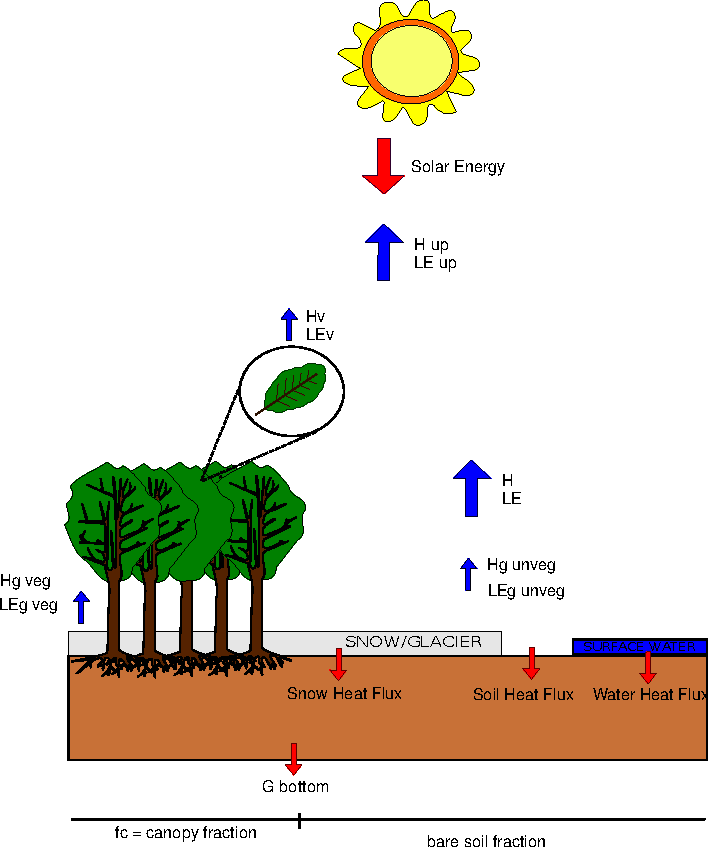
\includegraphics[width=1\textwidth]{./images/pic_surFlux/energy.pdf}
%    \textsl{\caption{Energy Budget} \label{}}
%  \end{minipage}
%\end{center}
%\end{figure}
